%
% Capítulo 3
%
\chapter{Architecture} \label{cap:architecture}

This chapter offers a comprehensive overview of the system's components and their interactions. It details the project's capabilities and presents the designed and developed architecture, entities, and implementation blueprint.

\section{Overview}

Figure ~\ref{fig:architecture} presents a diagram illustrating the main components of the system and their interactions. 

\begin{figure}[h]
	\begin{center}
		\resizebox{160mm}{!}{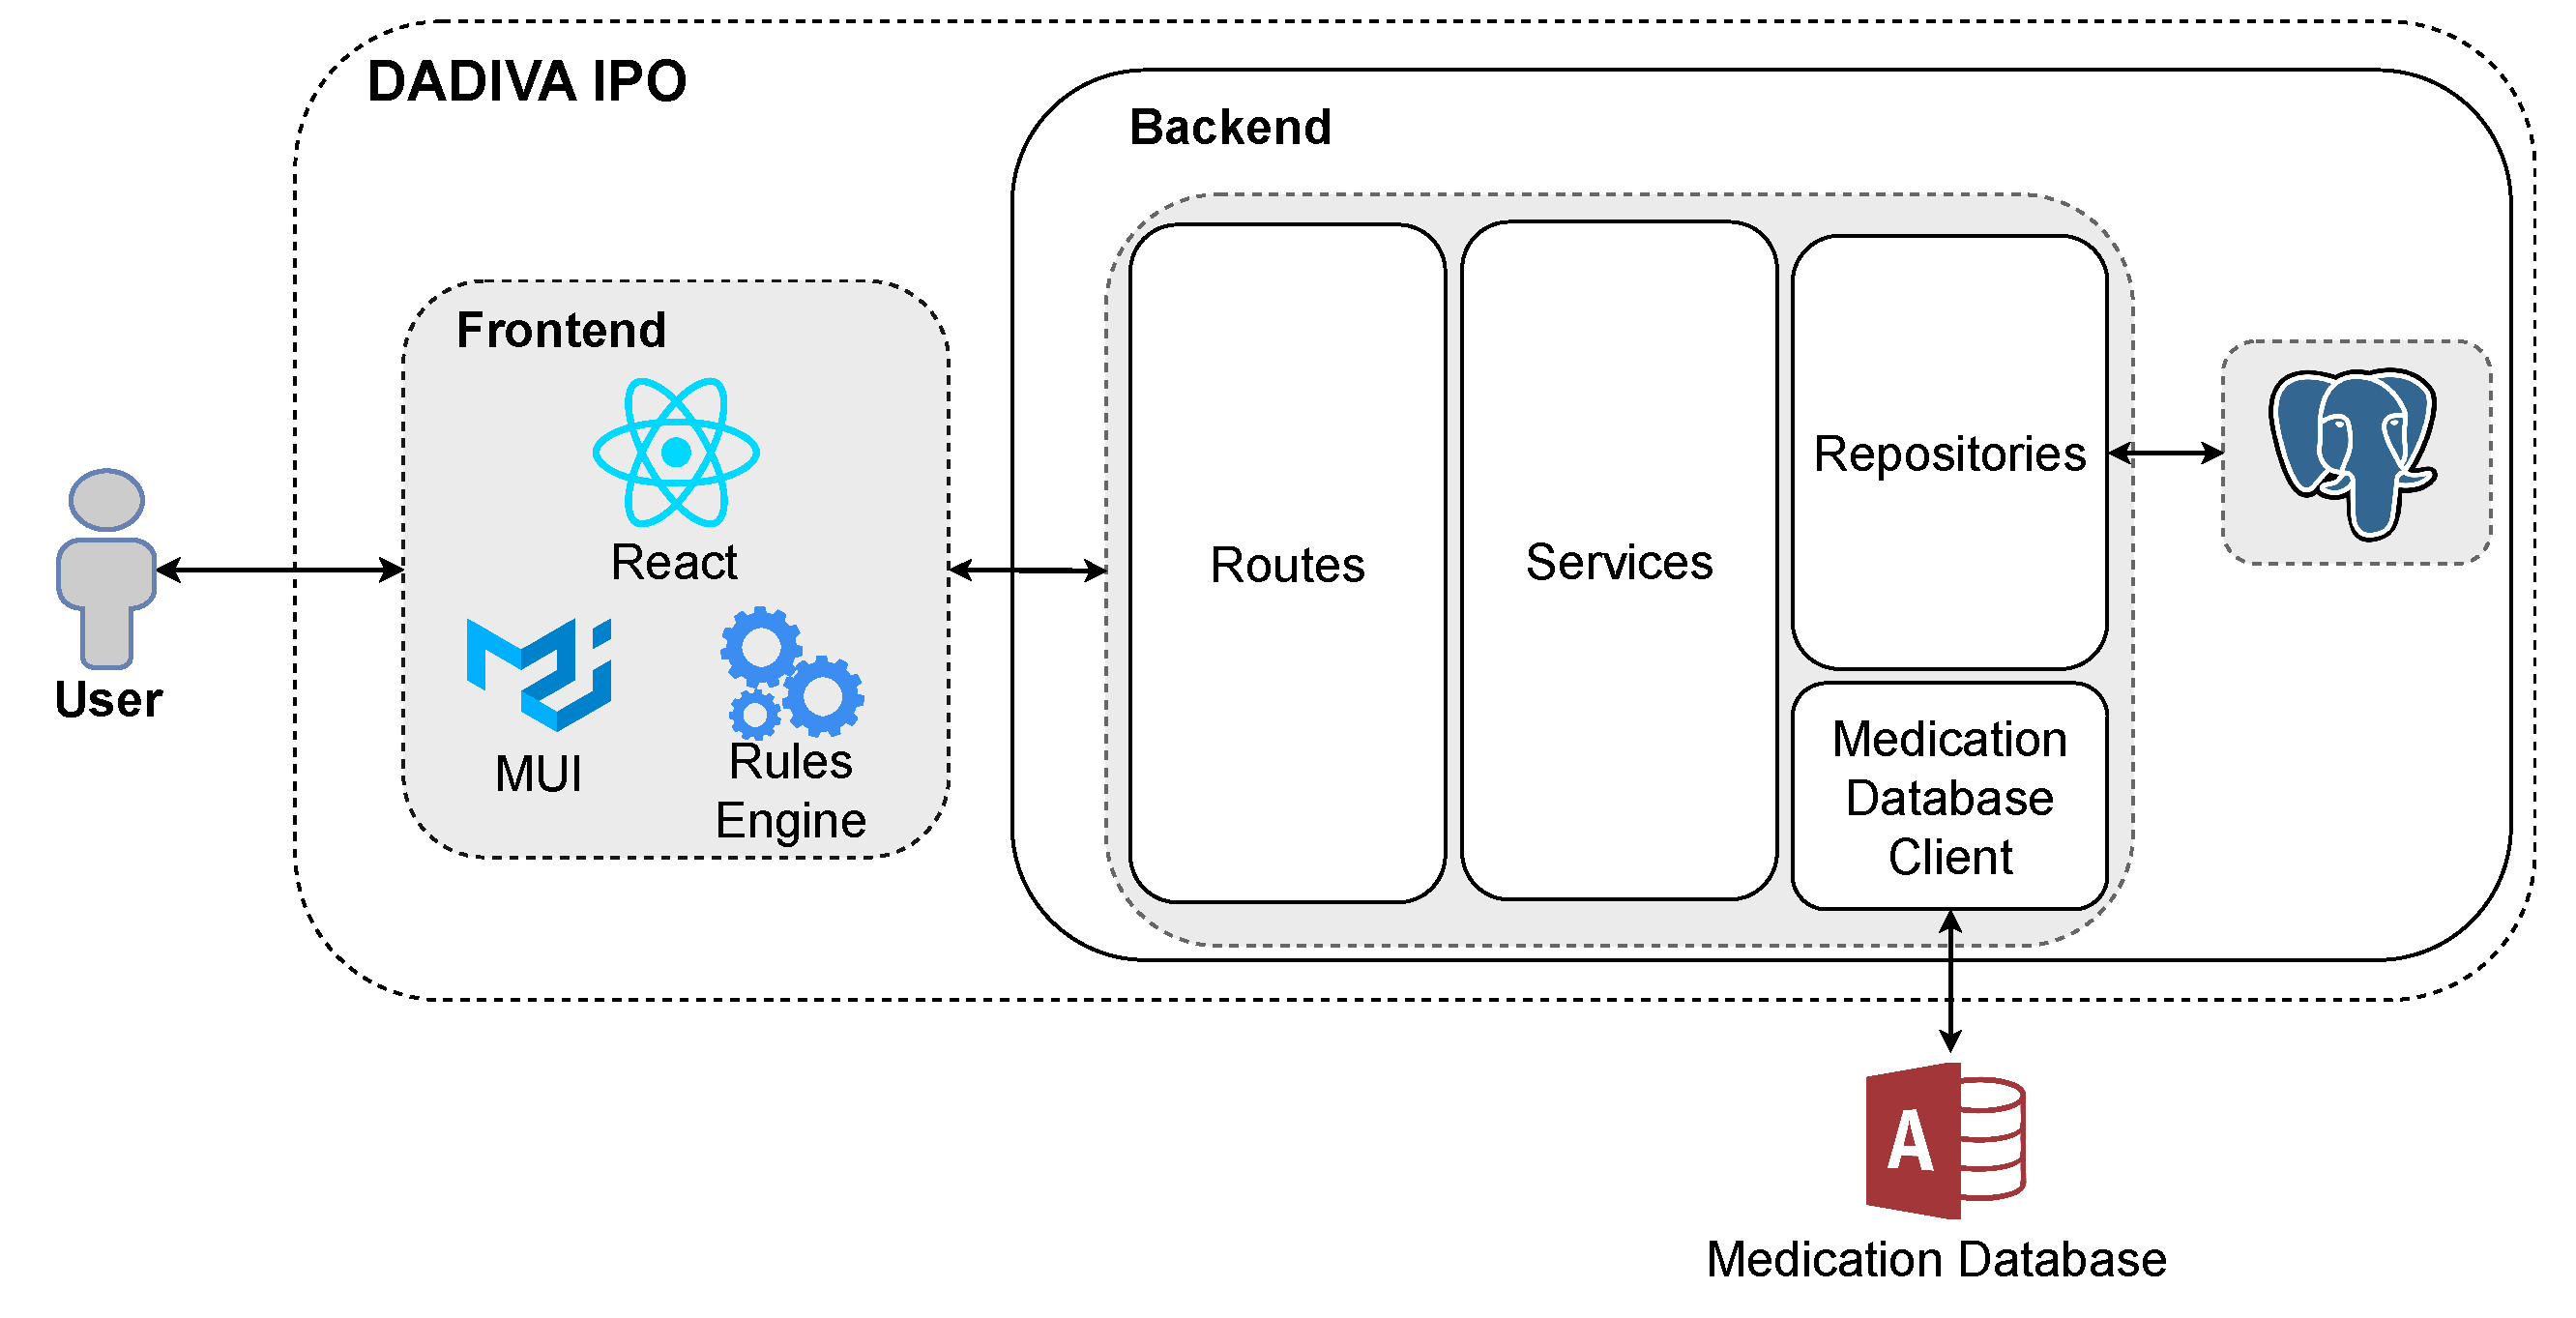
\includegraphics{./figures/Architecture.pdf}}
	\end{center}
	\caption{Application Architecture, gray squares represent containerized components of the solution.}\label{fig:architecture}
\end{figure}


The system consists of a backend application (server-side) and a frontend application (client-side).
The backend architecture consists of routes, services, repositories and a medication database client.
%The authentication server,  serves as a placeholder for future integration with AMA's authentication services.

The routes expose the backend's endpoints and handle incoming HTTP requests and call the appropriate service.

The services manage data manipulation, validation, and interact with the medication database client and the repositories layer.

The repository layer stores and retrieves information stored in a PostgreSQL database.
The medication database client is responsible for requesting data from IPO's medication database, supplied by Infarmed.






\section{Frontend Application}\label{architecture_frontend}

The frontend application is a web-based interface designed to facilitate seamless interaction between users and the backend system. It features a user-friendly and intuitive interface, catering to different types of users with specific functionalities:

\begin{itemize}
	\item Donor Users: Can fill out the current donation form;
	\item Doctor Users: Can search for pathology and medication interactions with blood donation and request form answers for specific users;
	\item Administrator Users: Can customize the current form, update pathology and medication interaction information, update the inconsistencies and manage users.
\end{itemize}

The application is organized into multiple pages and components, each serving distinct purposes. It utilizes Material UI, a popular React component library, to ensure a consistent and responsive user interface across these components. Material UI provides pre-built components and design elements that streamline the development process and enhance the application's visual appeal.

In addition to the user interface, the application includes a service layer responsible for communicating with the backend application through the REST API.

This chapter serves as an overview, for implementation details refer to chapter \ref{cap:frontend_implementation}.

\subsection{JSON-Rules-Engine and Form structure}\label{arc_jre}

As illustrated in figure \ref{fig:architecture} we used a rules engine in the frontend, more specifically the \textbf{JSON-Rules-Engine}, for the purpose of enforcing form rules.

Forms consist of a list of questions, divided into groups, and a set of rules, which are added to the engine instance. These rules are defined by conditions and events. When the engine runs all the conditions that are true will return their respective event.

Conditions can be categorized into \textbf{top-level conditions} and \textbf{condition properties}, following the types specified in the JSON-Rules-Engine library. \textbf{Top-level conditions} refer to logical operators, such as all, any, and not, while \textbf{condition properties} involve boolean evaluations, such as determining whether a given input equals a specified value.

\textbf{Top level conditions} refer to logical operators, more specifically all, any and not, meanwhile \textbf{condition properties} refer to a boolean evaluation, i.e. does a given input equal a certain value.

These rules are described in a JSON format, with an example illustrated in Figure \ref{fig:jre_diagram}.

\begin{figure}[h]
	\begin{center}
		\resizebox{160mm}{!}{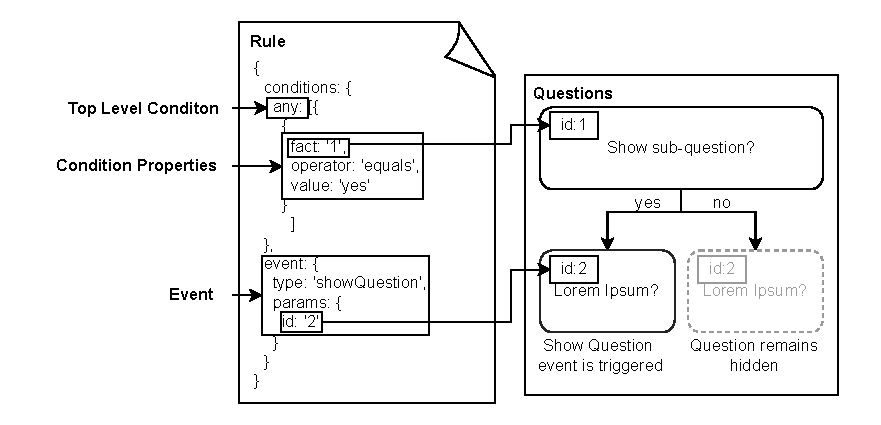
\includegraphics{./figures/JRE_diagram.pdf}}
	\end{center}
	\caption{JSON-Rules-Engine example with simple rule and question set.}\label{fig:jre_diagram}
\end{figure}

Note that the fact and value fields in the \textbf{condition properties} and the type and params fields for the \textbf{event} do not have predefined values. The use of a rules engine decouples rules from business logic, meaning the decision to link the fact and params fields to the ID of a question depends on the system implementation.
In our case we decided, not only that the before-mentioned fields would pertain to question Ids but also, that the type field for the \textbf{event} would have the following values:

\begin{itemize}
	\item \textbf{showQuestion:} show the question with id in the params field;
	\item \textbf{nextGroup:} allow for navigation to next group, is triggered when all the question in current group have been answered;
	\item \textbf{showReview:} allow form review, is triggered when all the answers in the form have been answered and donor can review form.
\end{itemize}

For implementation details, i.e. how the questions become visible and the rules are added to the engine, refer to section \ref{form_implementation}.
\newpage

\subsection{Mocks}
During planning some mockups where created of the final result for some pages, the login page is presented in Figure ~\ref{fig:login}, the form pages are presented in Figures ~\ref{fig:form},~\ref{fig:form_no} and ~\ref{fig:form_yes}, the backoffice page is presented in Figure ~\ref{fig:backoffice}.

\begin{figure}[H]
	\begin{center}
		\resizebox{160mm}{!}{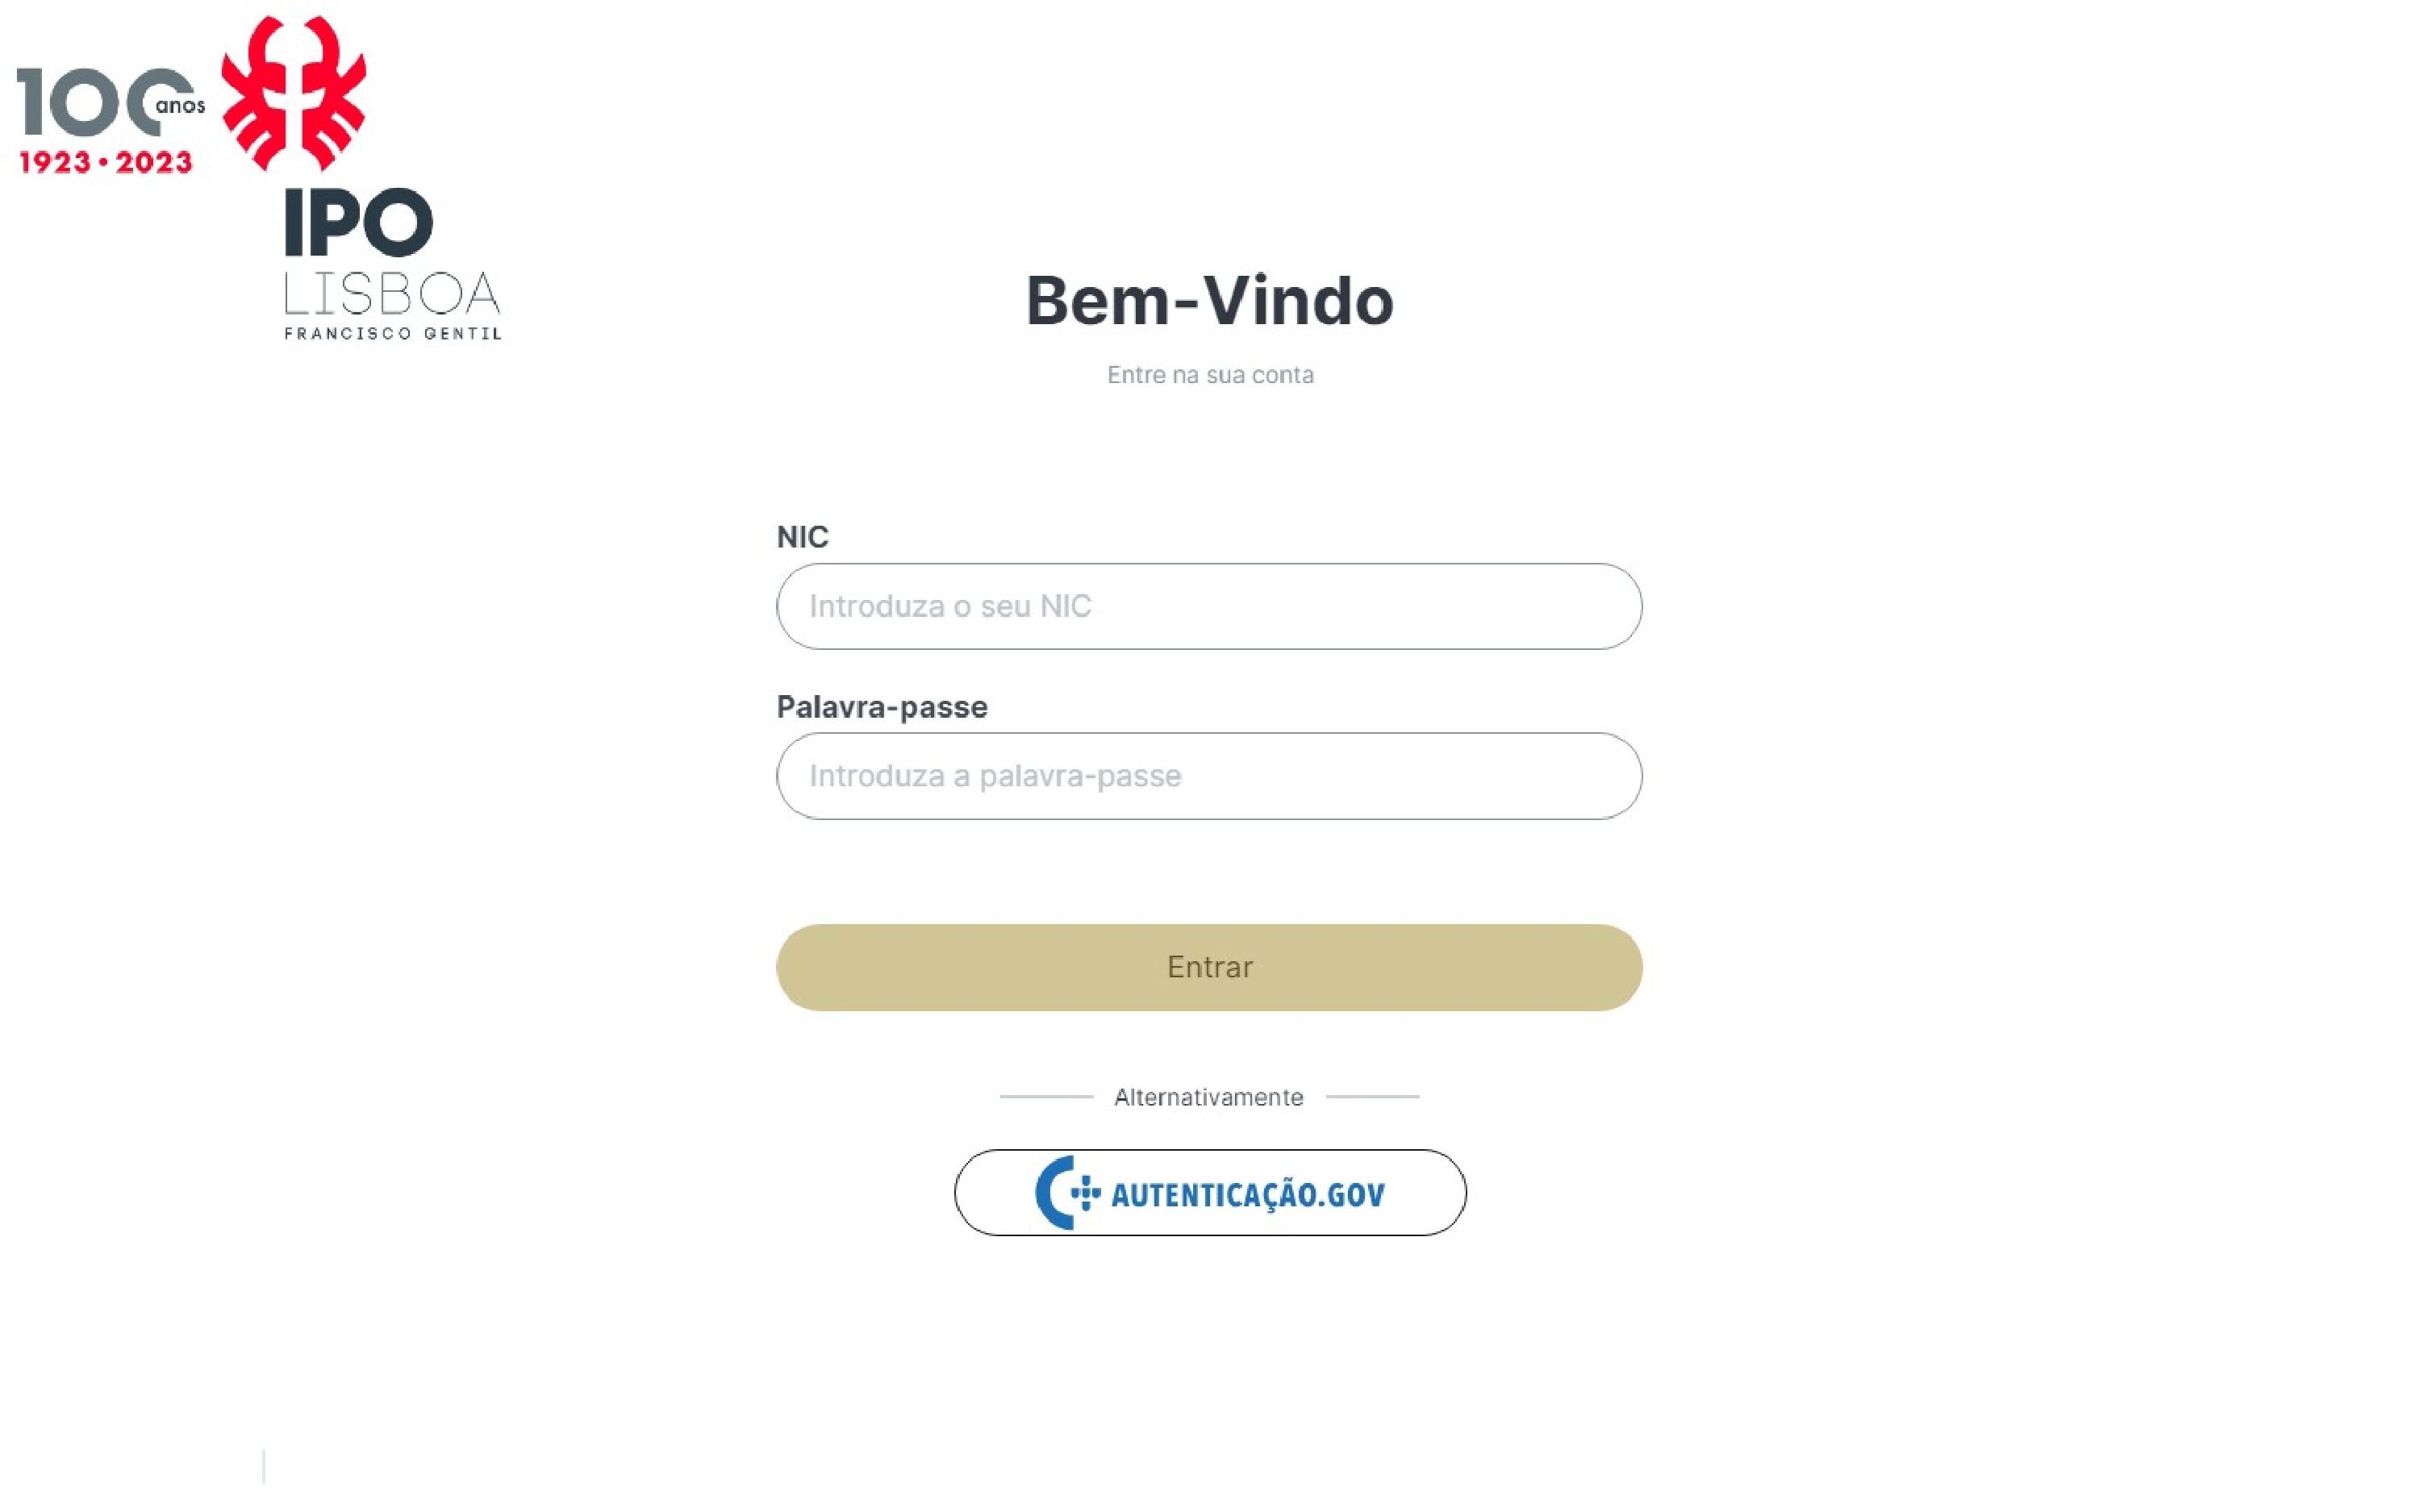
\includegraphics{./figures/Login.pdf}}
	\end{center}
	\caption{Login Page Mock.}\label{fig:login}
\end{figure}

\begin{figure}[H]
	\begin{center}
		\resizebox{160mm}{!}{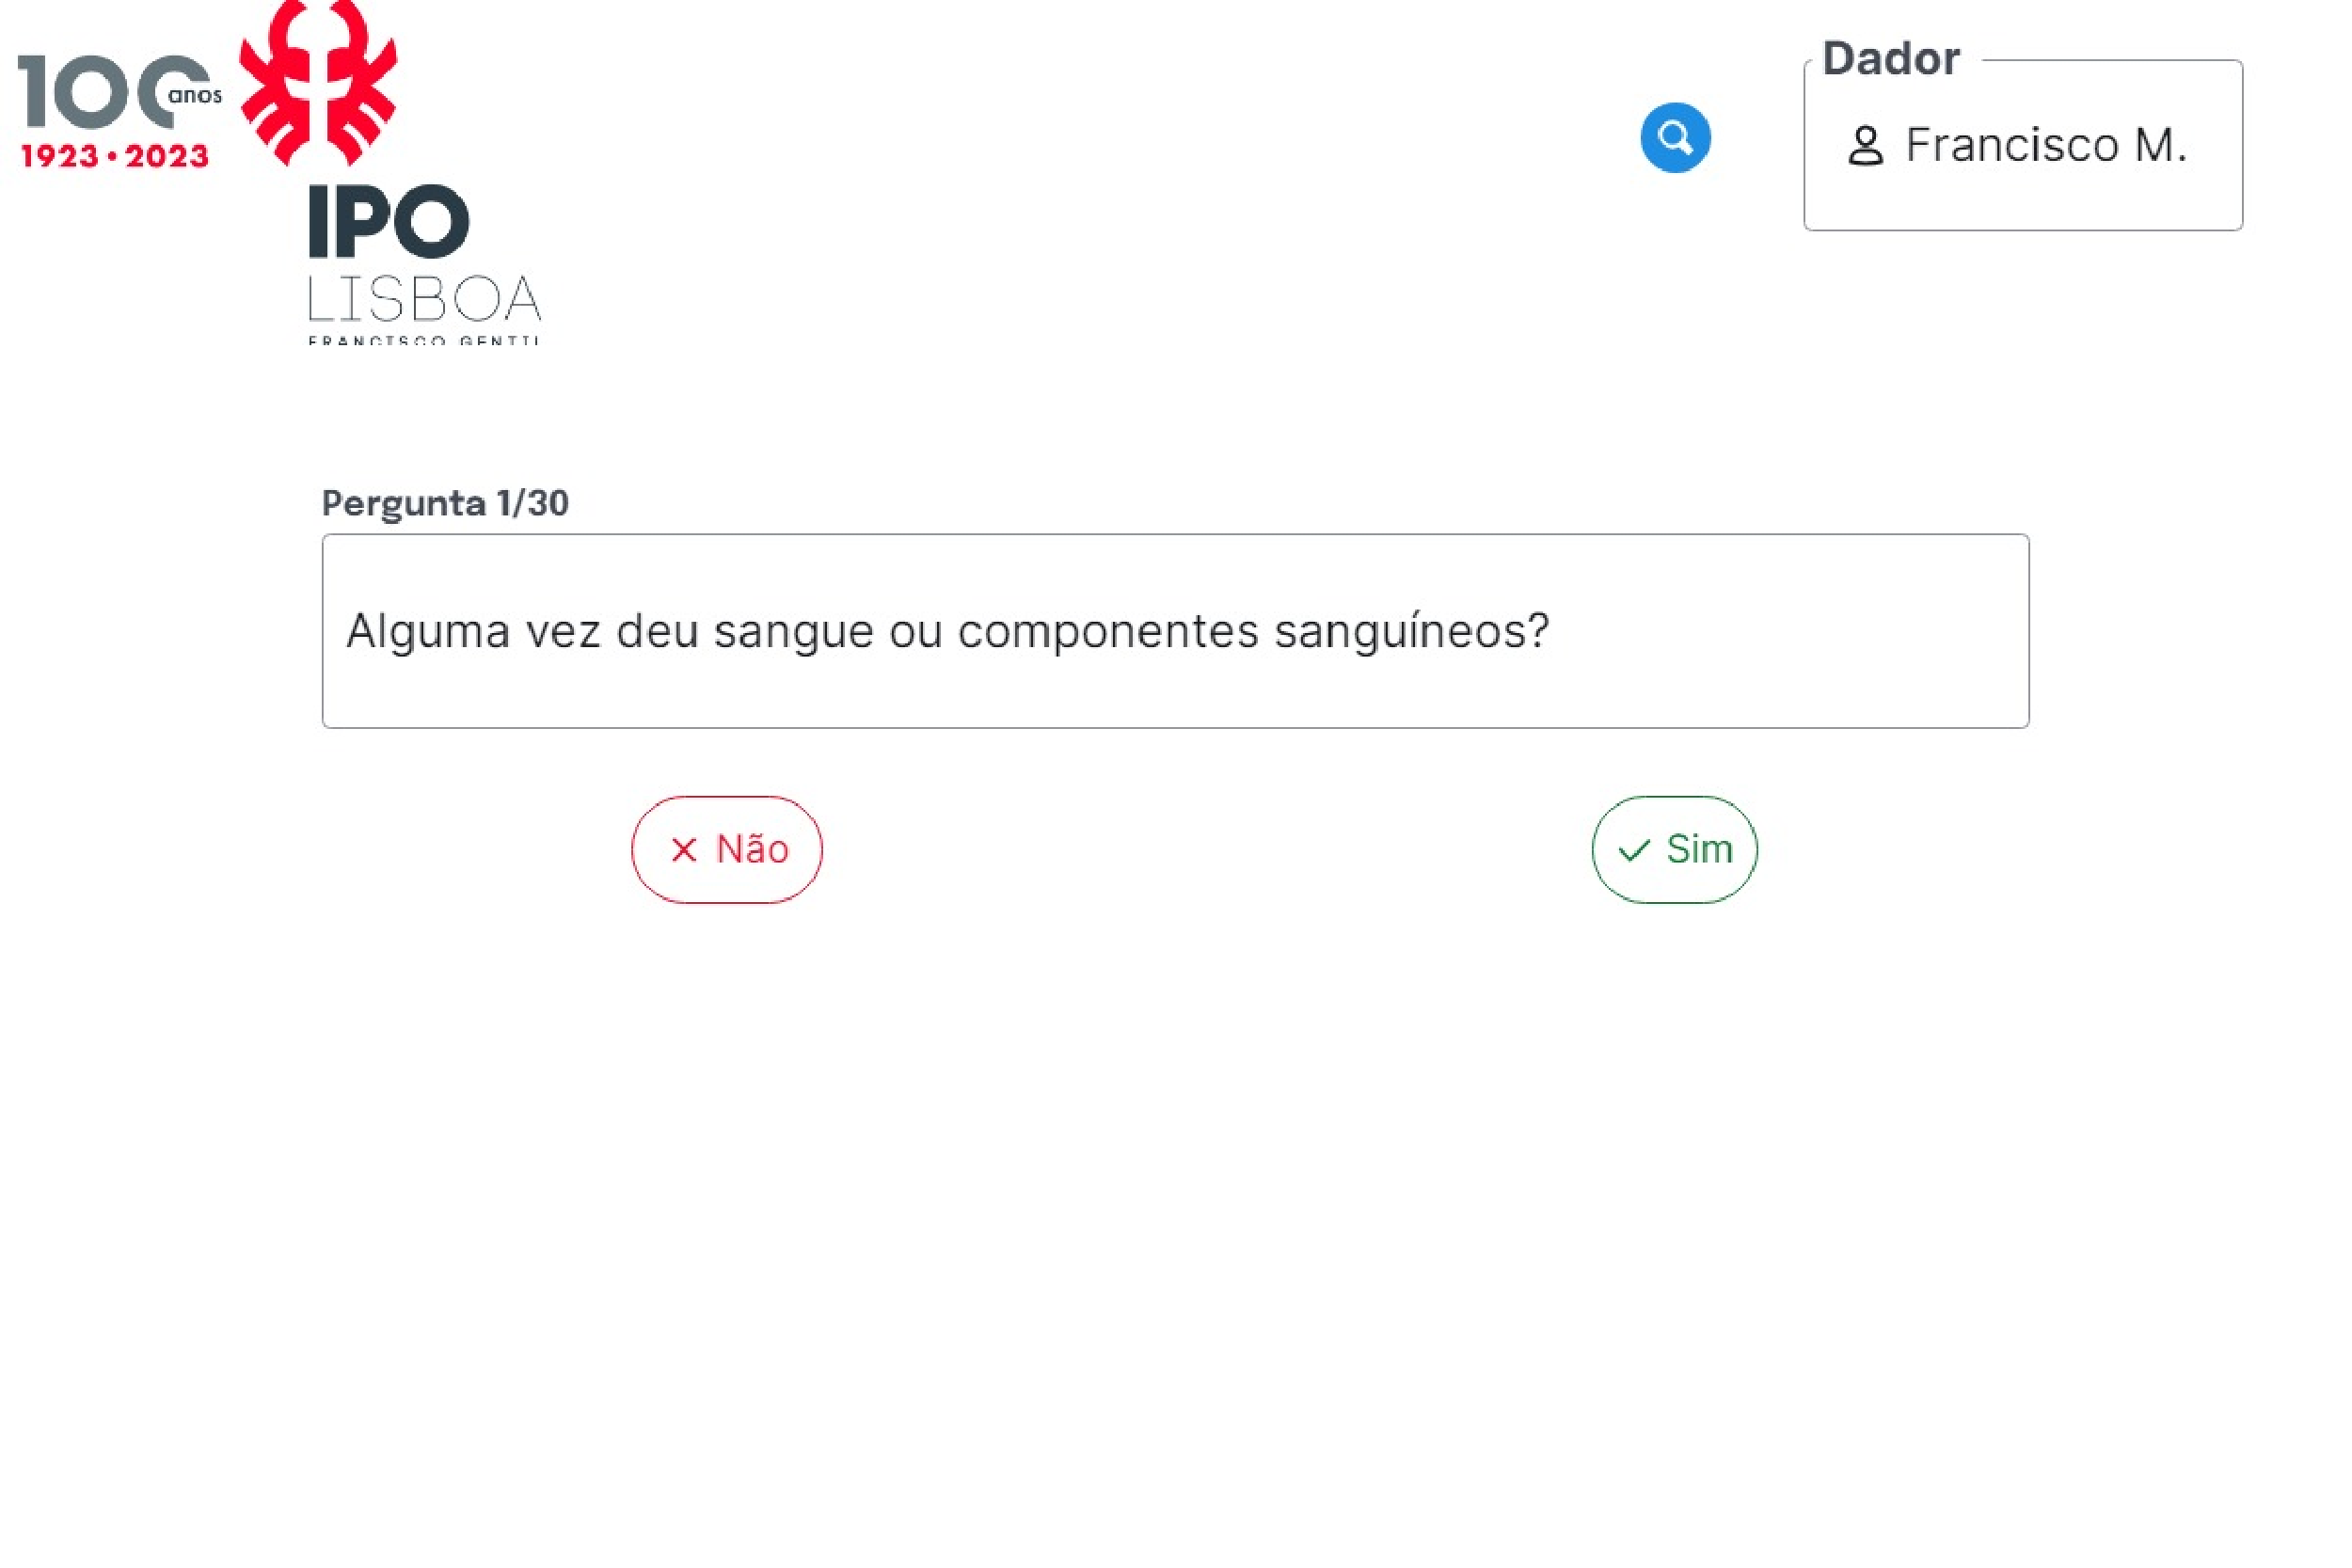
\includegraphics{./figures/Form.pdf}}
	\end{center}
	\caption{Form Page Mock.}\label{fig:form}
\end{figure}

\begin{figure}[H]
	\begin{center}
		\resizebox{160mm}{!}{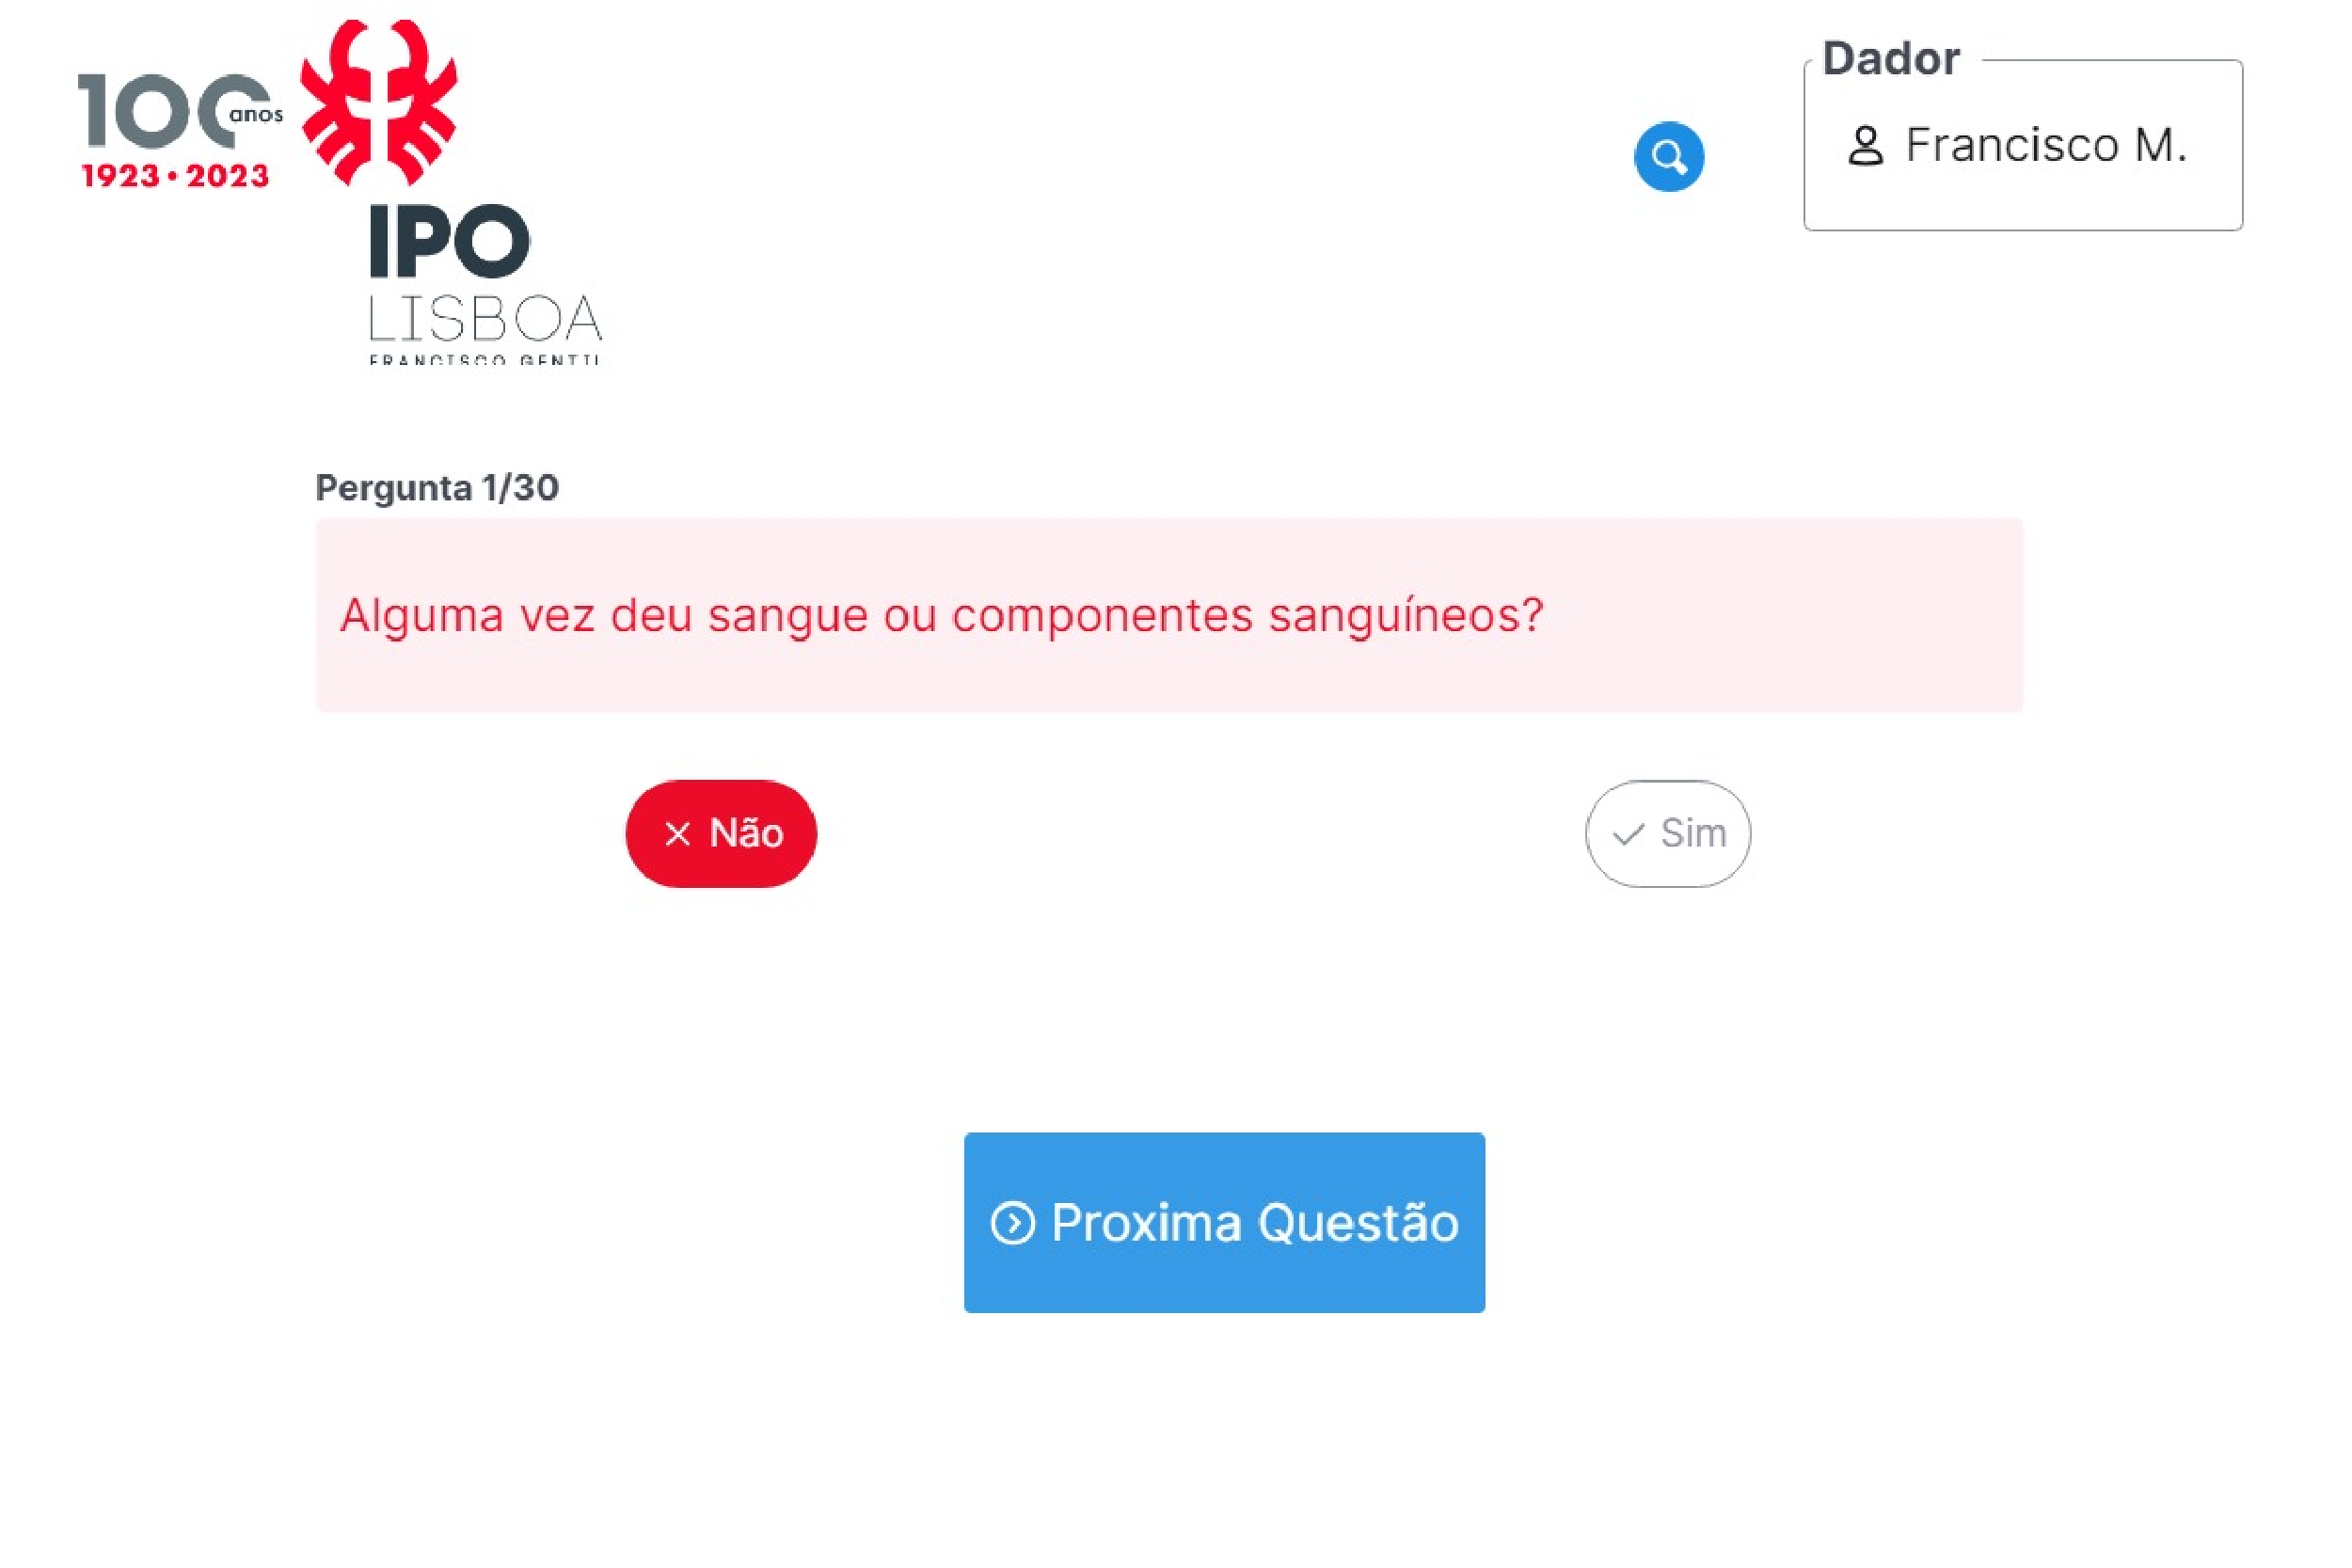
\includegraphics{./figures/Form_Answer_No.pdf}}
	\end{center}
	\caption{Form Page Negative Answer Mock.}\label{fig:form_no}
\end{figure}

\begin{figure}[H]
	\begin{center}
		\resizebox{160mm}{!}{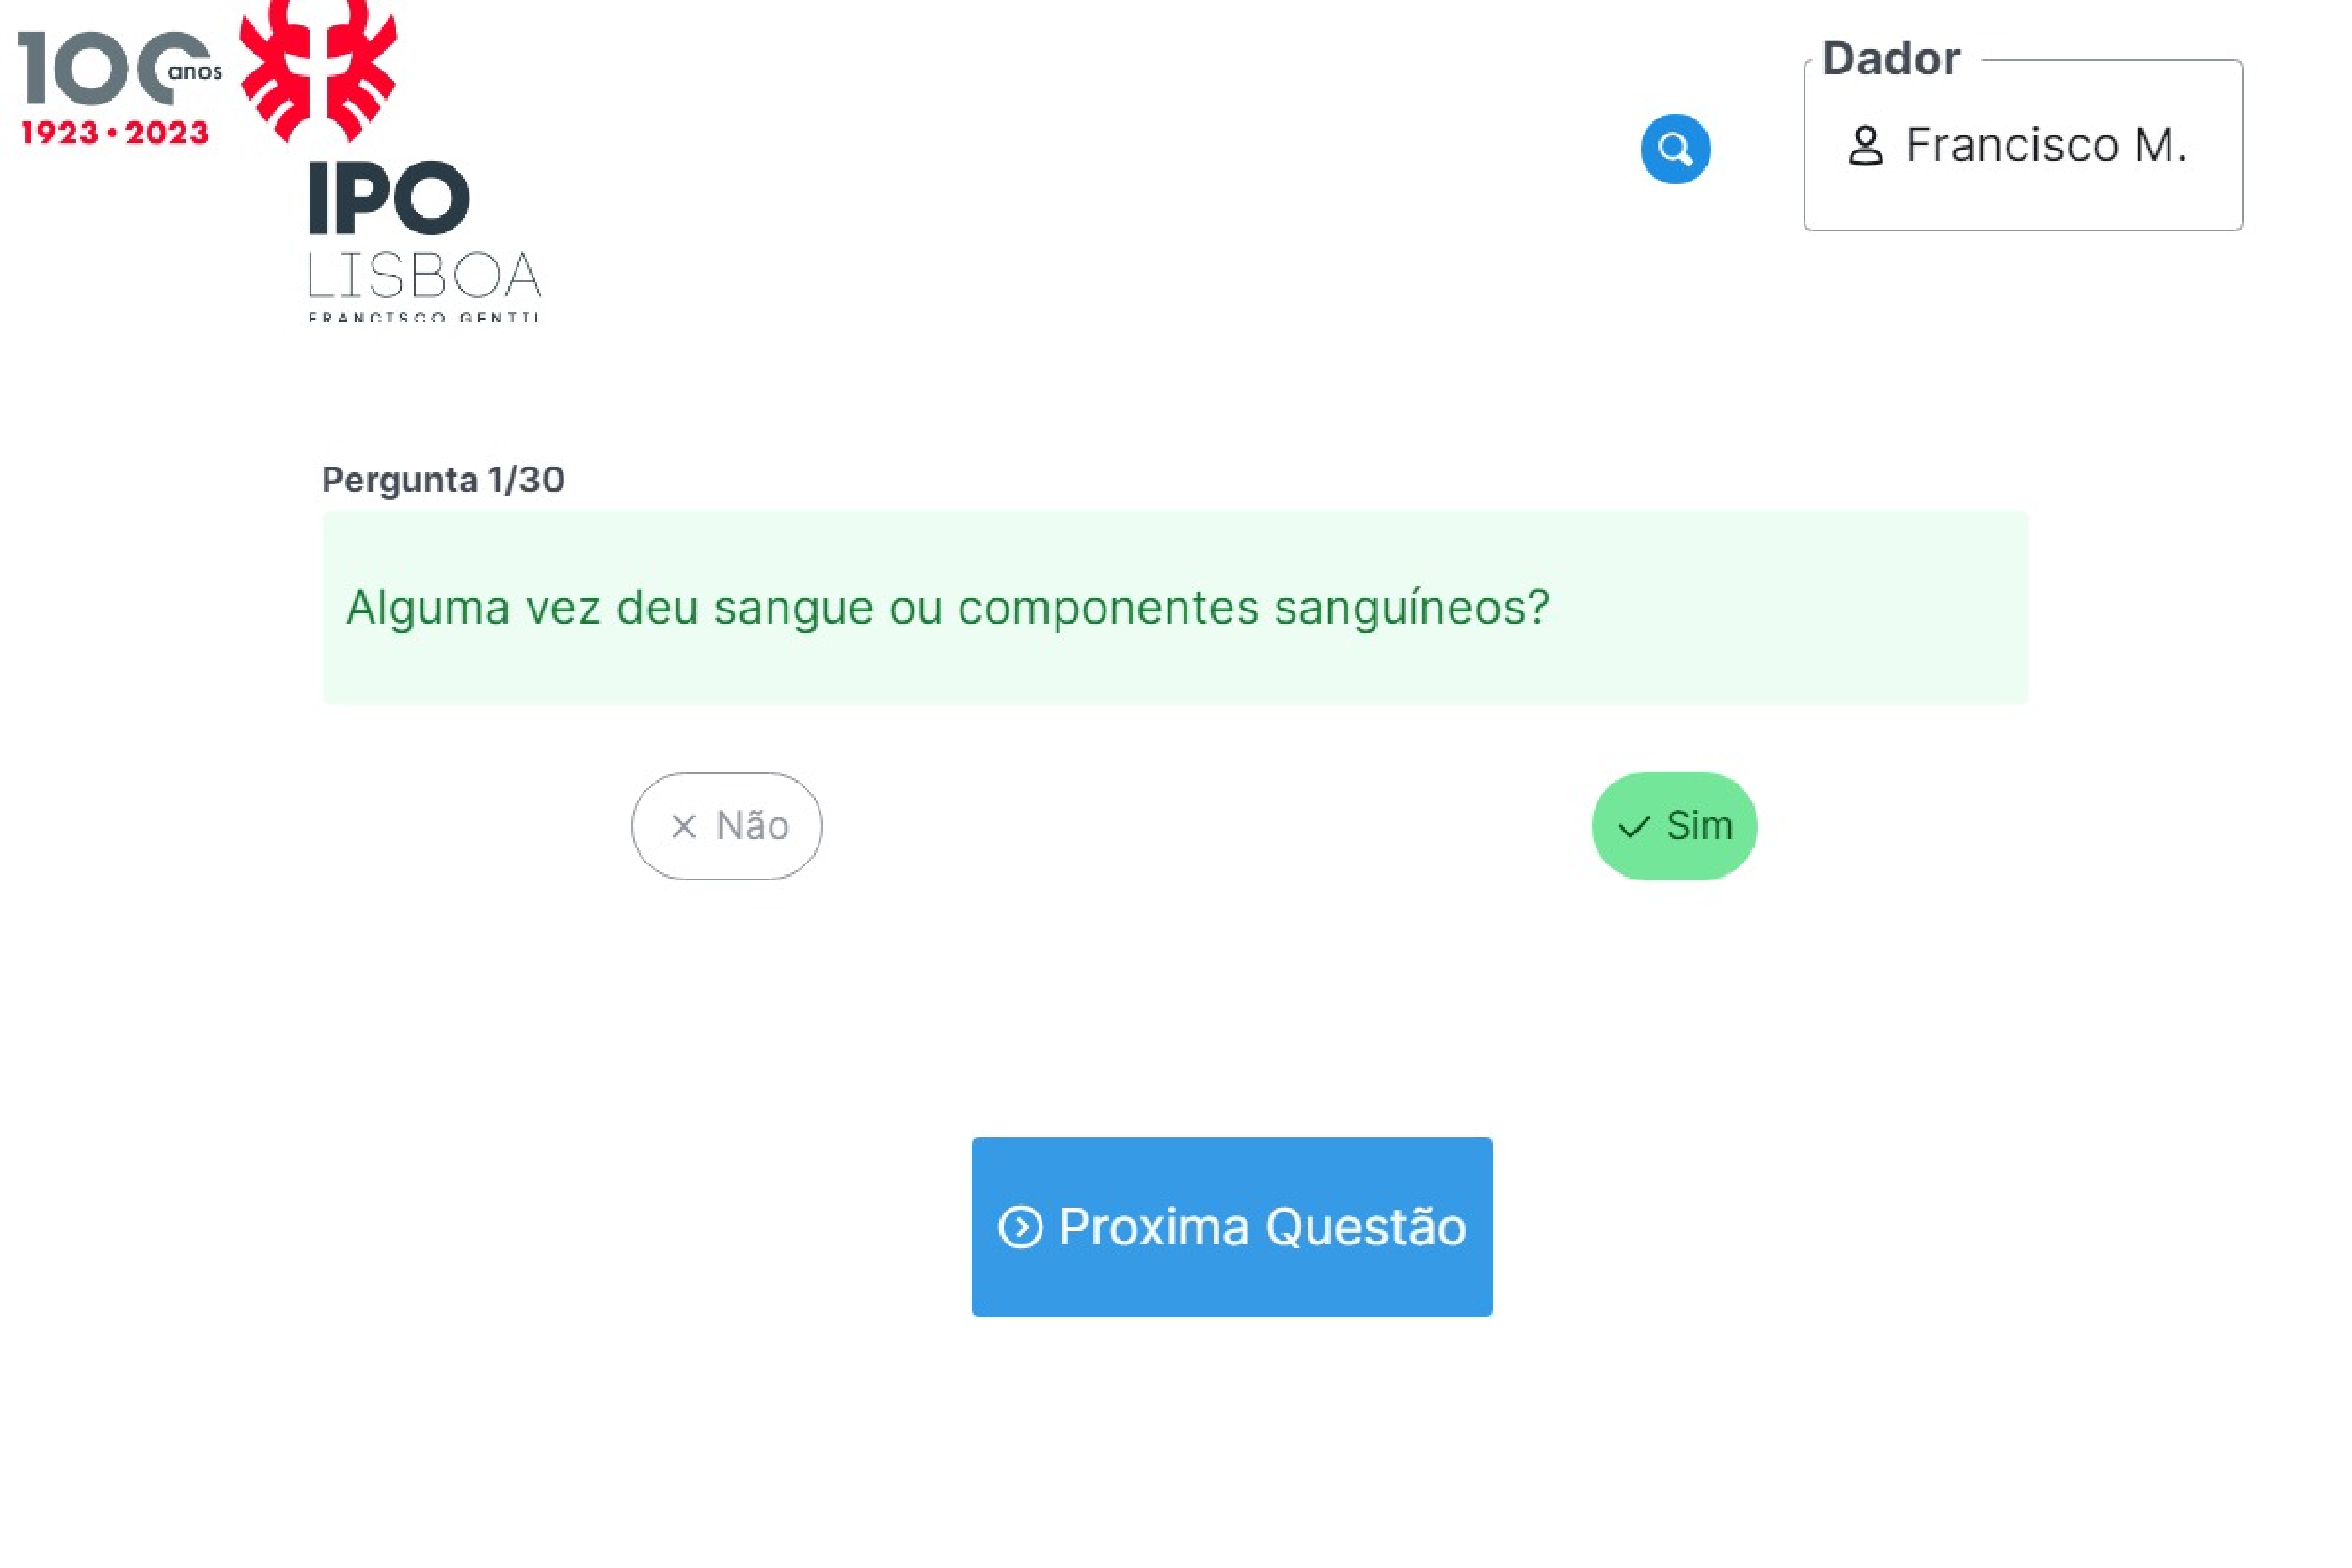
\includegraphics{./figures/Form_Answer_Yes.pdf}}
	\end{center}
	\caption{Form Page Positive Answer Mock.}\label{fig:form_yes}
\end{figure}

\begin{figure}[H]
	\begin{center}
		\resizebox{160mm}{!}{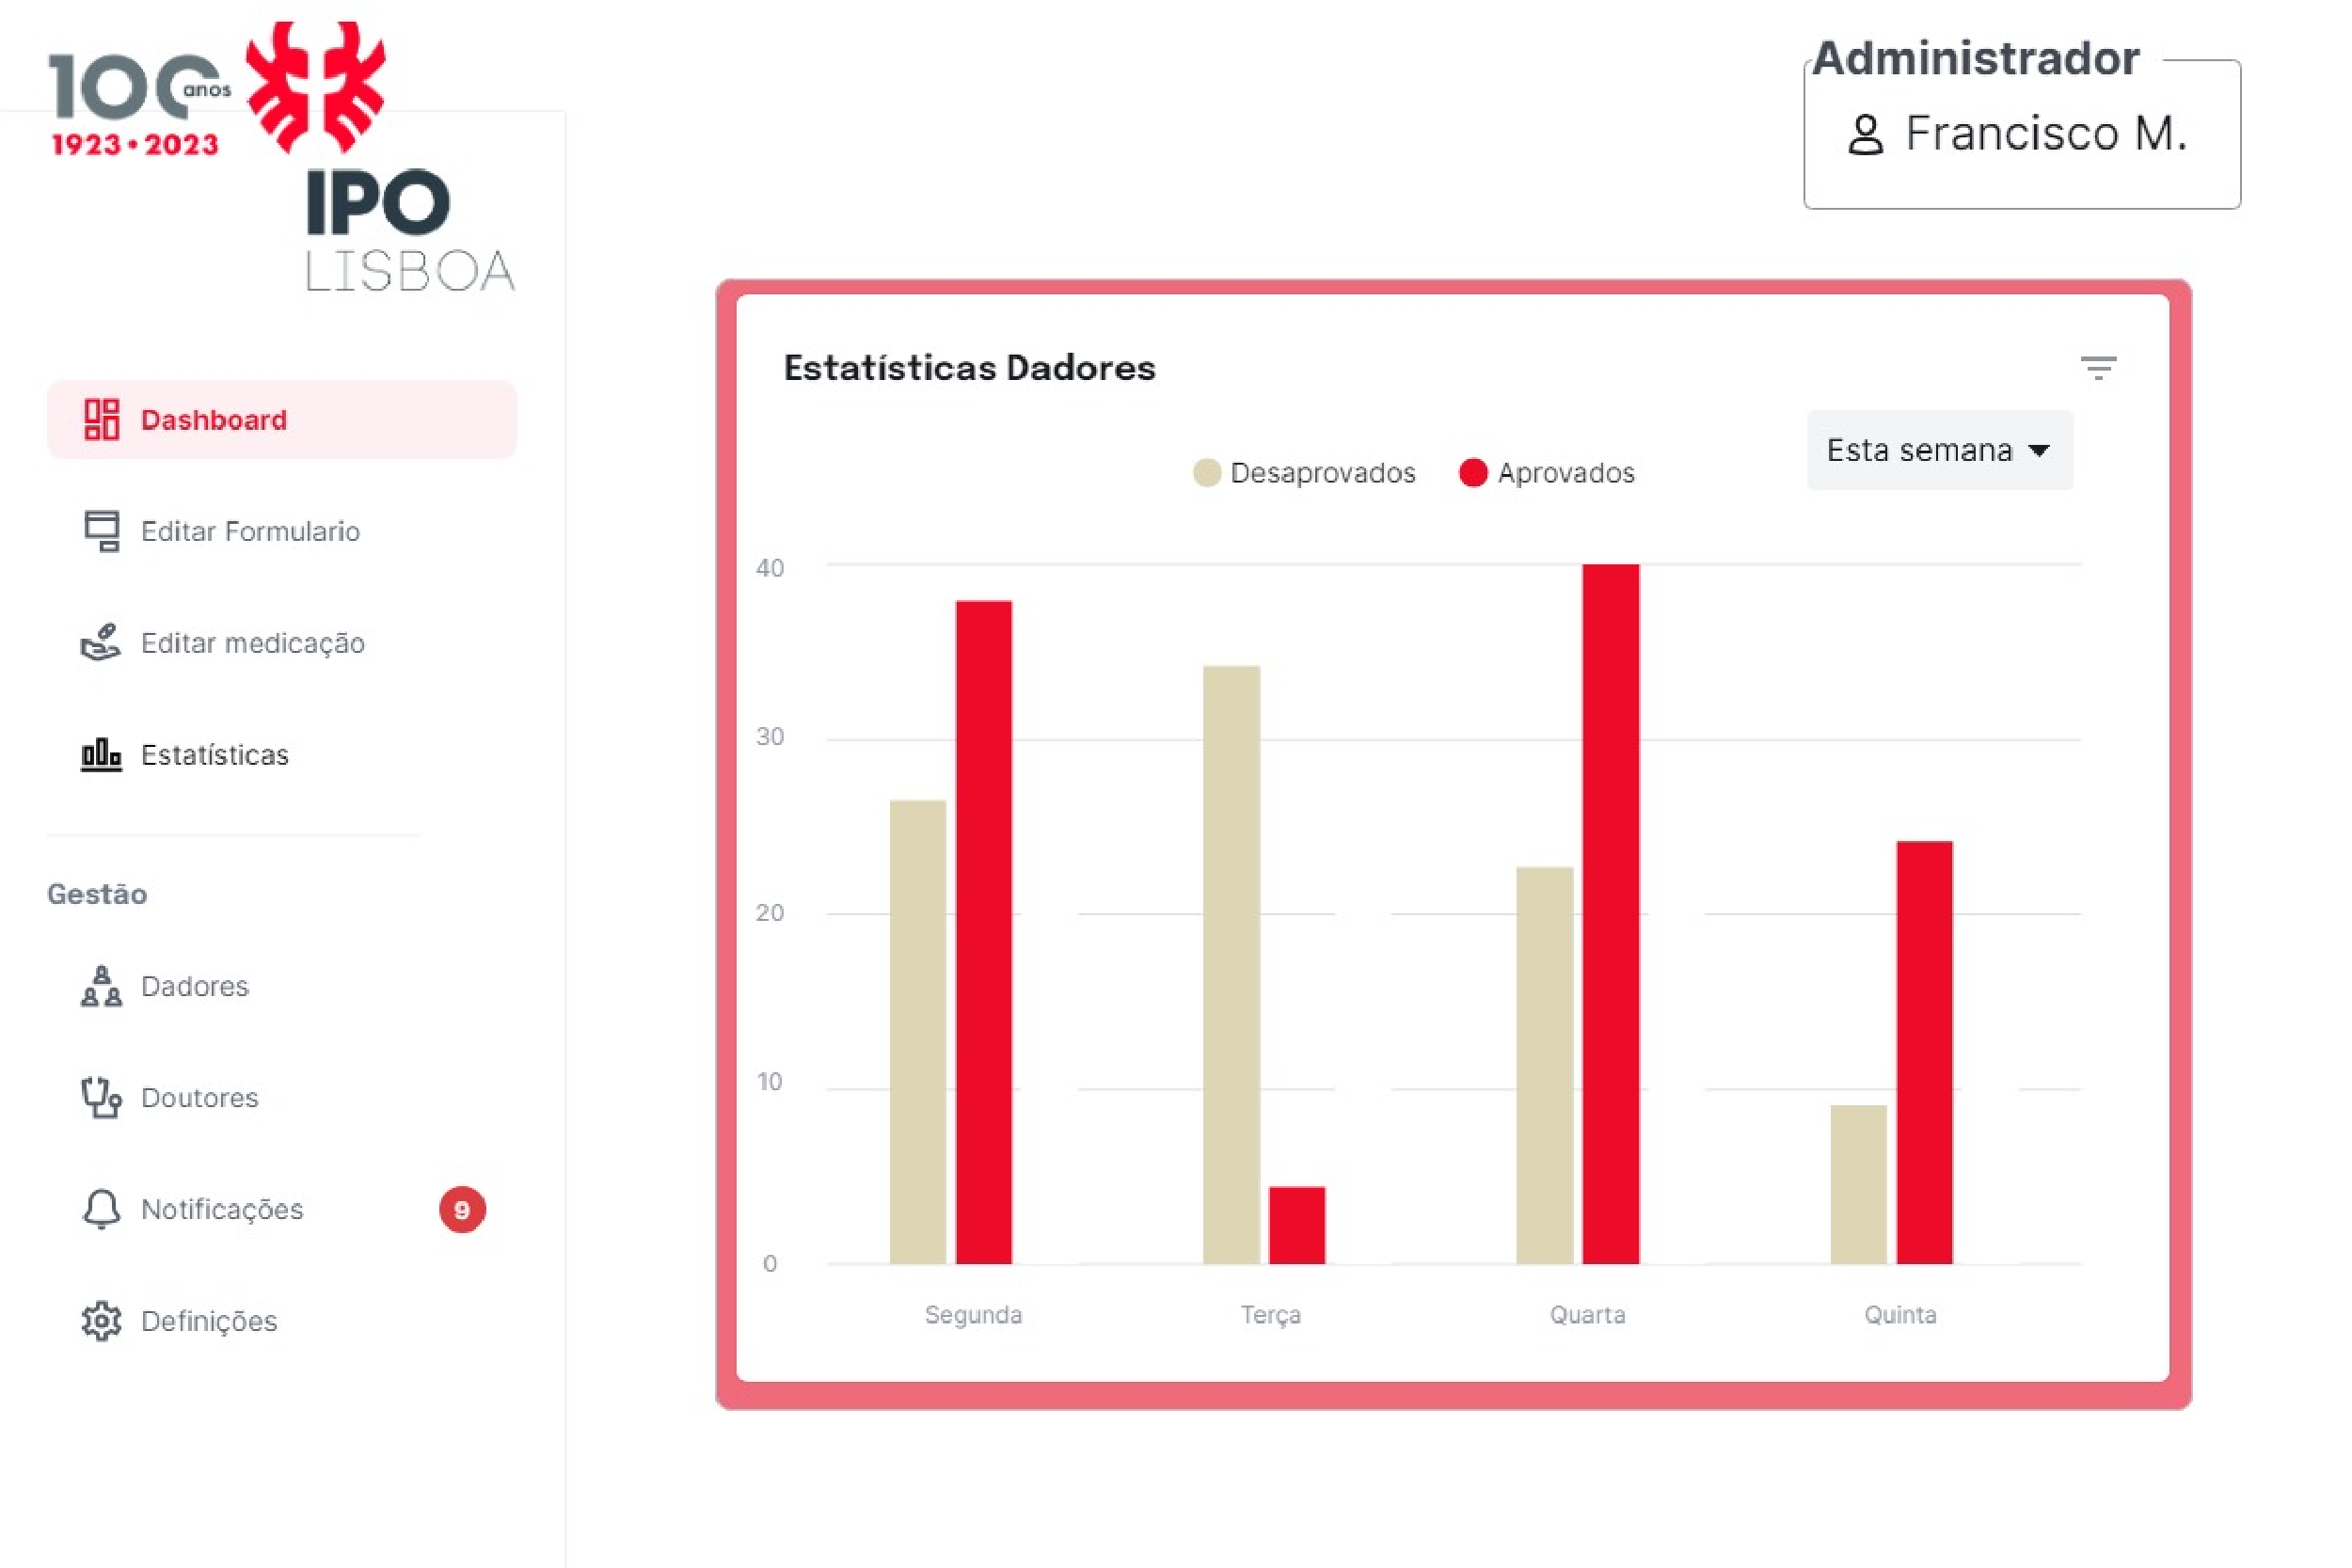
\includegraphics{./figures/Backoffice.pdf}}
	\end{center}
	\caption{Backoffice Page Mock.}\label{fig:backoffice}
\end{figure}

\newpage





\section{Backend Application}

The backend application can be abstracted into 4 layers:
\begin{itemize}
	\item Routes: responsible for receiving the http request and calling the correct service;
	\item Services: contains the services that manage the business logic of the application;
	\item Medication Database Client: responsible for requesting information to IPO's medication database;
	\item Repositories: contains the repository layer of the application;
\end{itemize}

With each one of these layers being divided by groups of functions that deal with a certain data model, such:
\begin{itemize}
	\item form;
	\item manual;
	\item medications;
	\item terms;
	\item submissions;
	\item review;
	\item users;
\end{itemize}

\subsection{Service Layer Error Handling}\label{service_layer_error_handling}

When an error occurs in the backend, it is crucial not to expose any sensitive information, such as the exception thrown. Exposing raw exceptions can lead to security vulnerabilities and may leak implementation details that could be exploited by malicious actors. To handle errors safely and effectively, we will utilize a \textbf{Result} class.

The \textbf{Result} class can represent two states: \textbf{Success} or \textbf{Problem}.
\begin{itemize}
	\item \textbf{Success}: This state indicates that the request was processed successfully. It encapsulates the result of the operation, ensuring that the expected outcome is communicated clearly to the client.
	\item \textbf{Problem}: This state is defined in accordance with RFC 7807\cite{rfc7807}. The \textbf{Problem} class provides a standardized way to convey error information. It ensures that detailed error information is supplied without exposing sensitive data. By following the RFC 7807 specification, the Problem class includes the following fields:
	\begin{itemize}
		\item \textbf{'type'}: A URI reference that identifies the problem type. This URI is intended to provide human-readable documentation for the specific problem encountered.
		\item \textbf{'title'}: A short, human-readable summary of the problem type. This remains consistent across occurrences of the same problem type, making it easier for developers to recognize recurring issues.
		\item \textbf{'status'}:  The HTTP status code generated by the origin server for this particular occurrence of the problem. This aligns with standard HTTP status codes, facilitating easy interpretation by both humans and machines.
		\item \textbf{'details'}: A human-readable explanation specific to this instance of the problem. It provides more context and helps in understanding the error without revealing sensitive information.
	\end{itemize}
\end{itemize}

The \textbf{Problem} class's standardized format ensures that error information is conveyed consistently, which enhances both the readability for humans and the parsability for machines. This consistency is vital for effective debugging, logging, and automated error handling.

When possible the 'title' and 'details' fields should follow some guideline to ensure security, such as owasp's recommendation for authentication error responses \cite{owasp_authentication}, which states that "using any of the authentication mechanisms (login, password reset, or password recovery), an application must respond with a generic error message regardless of whether:The user ID or password was incorrect.The account does not exist.The account is locked or disabled."

An example of the flow for GET form resource request is presented in Figure ~\ref{fig:getForm_Sequence_Diagram}

\begin{figure}[h]
	\begin{center}
		\resizebox{160mm}{!}{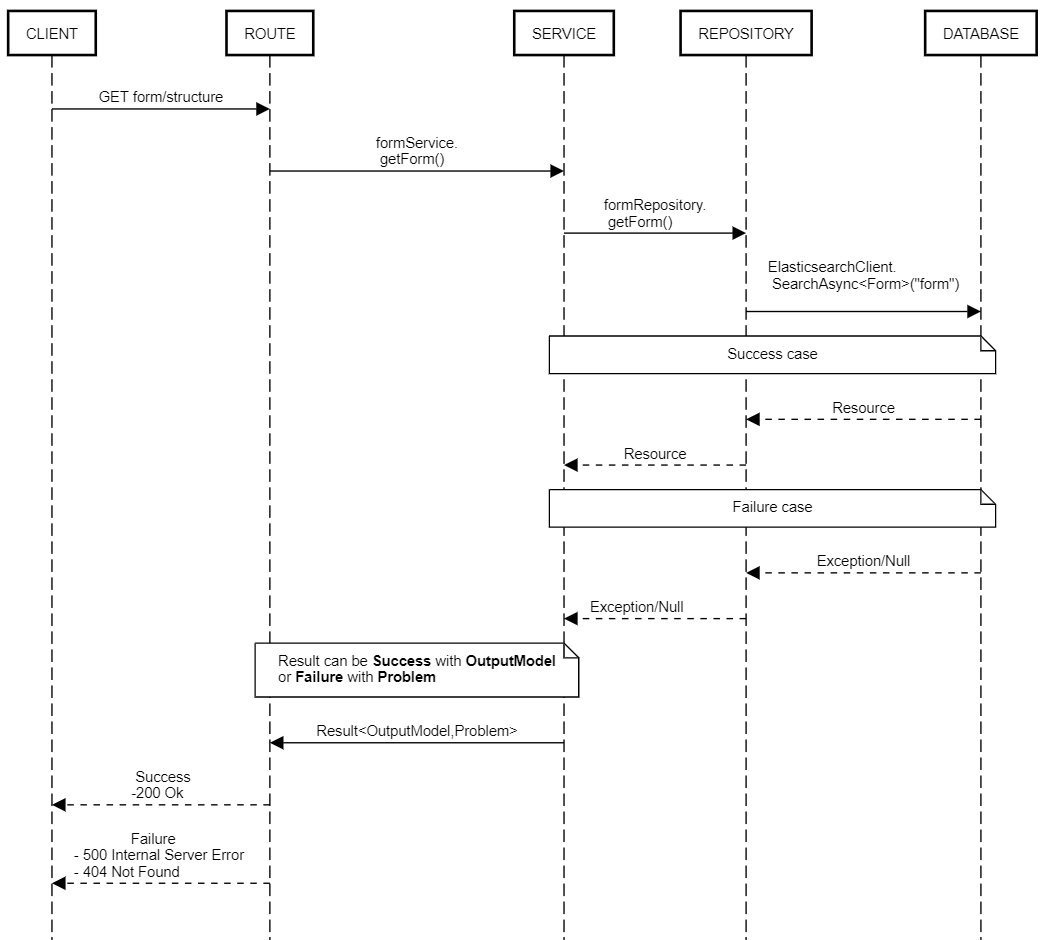
\includegraphics{./figures/getForm_Sequence_Diagram.png}}
	\end{center}
	\caption{Get Form Sequence Diagram.}\label{fig:getForm_Sequence_Diagram}
\end{figure}








%The backend handles HTTP requests directed to specific endpoints. The route associated with each endpoint converts the request body into an appropriate model, if necessary, and then calls the corresponding service, passing along the model. The service validates the model, converts it into a domain object, and calls the relevant repository. Using an ElasticClient, the repository stores the object in the ElasticSearch database. The appropriate response is then propagated back up, as illustrated in Figure ~\ref{fig:backendLayers}.
%
%\begin{figure}[H]
%	\begin{center}
	%		\resizebox{100mm}{!}{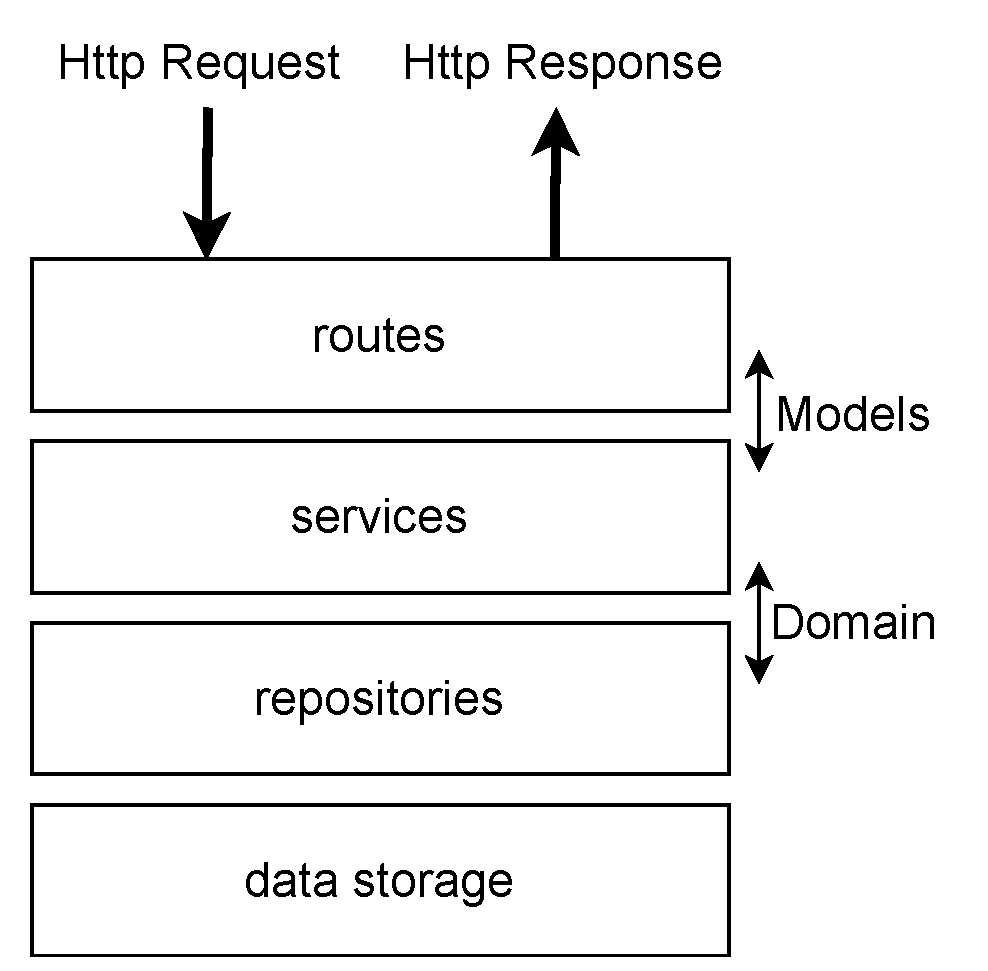
\includegraphics{./figures/backendLayers.pdf}}
	%	\end{center}
%	\caption{Backend layers.}\label{fig:backendLayers}
%\end{figure}




%\section{Form Data Model and Inconsistencies Data Model}

%The first approach to solve the dynamic form challenge was to use a data structure formed by pairs of main questions and sub-questions, example presented in Figure ~\ref{fig:old_form}, where a main question can only be answered with boolean values, and one of those values triggers the display of a sub-question which has a certain type of response, such as boolean, dropdown for known multiple answers, and text, to accept user text input.

%\begin{figure}[hbt!]
%	\begin{center}
	%		\resizebox{150mm}{!}{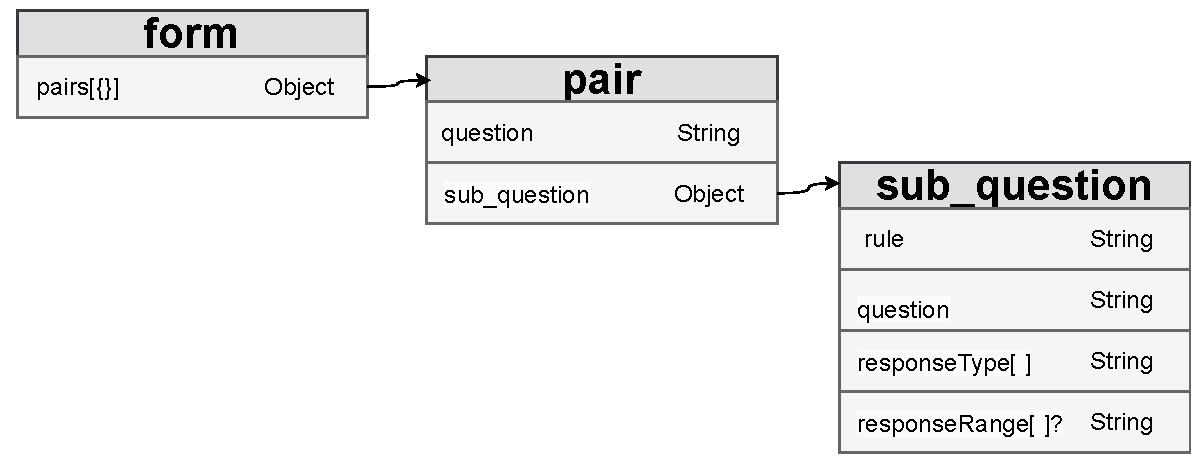
\includegraphics{./figures/oldForm.pdf}}
	%	\end{center}
%	\caption{First Form Data Structure.}\label{fig:old_form}
%\end{figure}
%
%This approach has several drawbacks. Firstly, it prevents the suppression of further questions, which contradicts the goal of creating a flexible and adaptable solution. Additionally, it conflates questions and rules within sub-questions, leading to a lack of clarity and potential confusion in implementation.
%
%Upon further discussion we settled on using a more complex data structure , exemplified in Figure ~\ref{fig:new_form}, composed by a list of questions and a list of rules.
%
%Each question has an id, the text that composes it, the type of response (boolean, text and dropdown) and can have options that lists all the possibles values for a multiple(dropdown) response.
%
%Each rule has conditions, which can be "any","all" or "not", so that, when any, all or none of the conditions are met an event is triggered.
%Each condition type will have a fact, an operator and a value. In essence, when a question, which is identified by the fact field via it's id, is answered a condition can true or false depending on the logical operator used, ie equal or notEqual, and the value of the answer. If the condition is true an event is triggered, this event can be to show or hide a subsequent question, this targeted question is identified via the id, supplied in the params field.
%
%This model, specifically the rules field, was chosen as it is part of the JSON-Rules-Engine specification, which is presented in more detail in Chapter ~\ref{cap:technologies} and is easily stored and retrieved in a ElasticSearch database.
%
%\begin{figure}[htbp]
%	\begin{center}
	%		{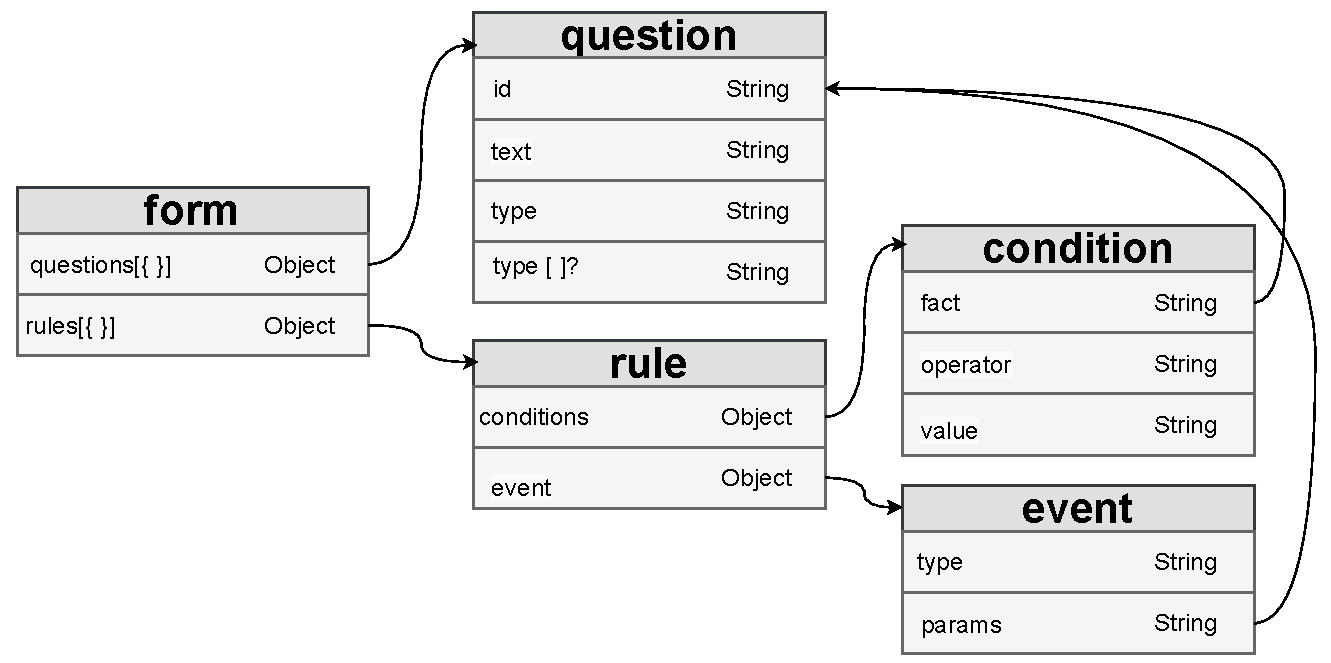
\includegraphics[width=\textwidth,height=\textheight,keepaspectratio]{./figures/newForm.pdf}}
	%	\end{center}
%	\caption{Final Form Data Structure.}\label{fig:new_form}
%\end{figure}
%\FloatBarrier
%
%The inconsistencies data model is compromised of rules, and describes answer combinations that are logical fallacies, ie a donor answering that they're healthy in one question and that they have a chronic disease in another question.
%
%\section{Submission Data Model}
%
%The submission data structure represents and answered form, has such it contains a list of answered questions, each answered question is composed by the question id and the answer, as referenced in Figure ~\ref{fig:submission_data_model}.
%
%\begin{figure}[hbt!]
%	\begin{center}
	%		\resizebox{150mm}{!}{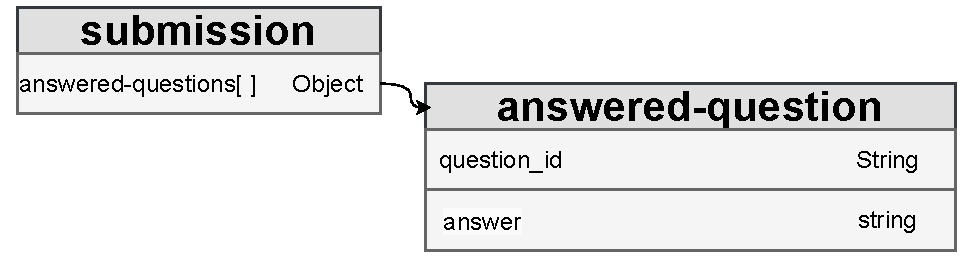
\includegraphics{./figures/Submission_Data_Model.pdf}}
	%	\end{center}
%	\caption{Submission Data Structure.}\label{fig:submission_data_model}
%\end{figure}
%
%
%\section{User Data Model}
%
%The user data structure is composed on an unique identifier, the nic, and the user hashed password, as referenced in Figure ~\ref{fig:user_data_model}.
%
%\begin{figure}[hbt!]
%	\begin{center}
	%		\resizebox{150mm}{!}{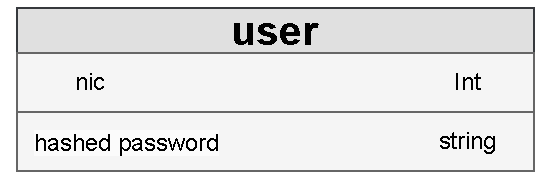
\includegraphics{./figures/User_Data_Structure.pdf}}
	%	\end{center}
%	\caption{User Data Structure.}\label{fig:user_data_model}
%\end{figure}

%%secalhar é mais adequado na descrição do problema




%\subsection{Form Services}
%
%The form service is responsible for managing the form resources.
%Figure ~\ref{fig:form_services} is a diagram that shows the architecture of the form services.
%
%\begin{figure}[htbp]
%	\begin{center}
%		\resizebox{150mm}{!}{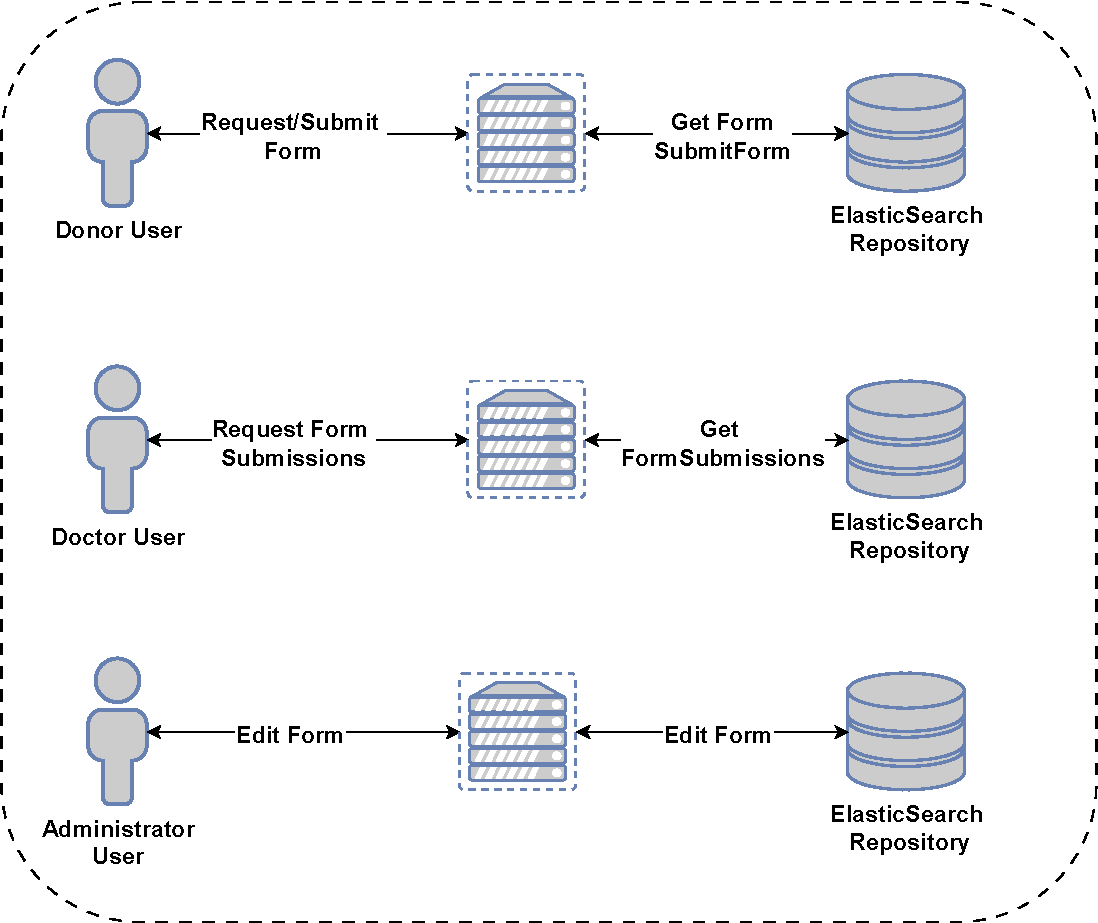
\includegraphics{./figures/formServices.pdf}}
%	\end{center}
%	\caption{Final Form Data Structure.}\label{fig:form_services}
%\end{figure}
